
% Szakdolgozat, diplomaterv esetén a dolgozat felépítése valami ehhez hasonló, témától függetlenül lehet természetesen eltérés:
% -Bevezetés, 1-2 oldal, a téma elhelyezése, miről lesz szó
% -Szakirodalmi áttekintés: a dolgozat kb harmada, szükséges előismereteket tartalmazza, illetve szakdolgozat esetén kb 5, diplomaterv esetén kb 10 szakmai cikk hivatkozása, 
%   1-1 bekezdésben összefoglalva, kik, mivel mit csináltak, milyen eredményre jutottak, az aktuális dolgozathoz hogy kapcsolódik, 
%   miért releváns. Kutatós témák esetén ez lényegesen nagyobb hangsúlyt kap (több cikk is hivatkozható!), 
%   fejlesztős feladatok esetén hasonló termékek bemutatása, elmélet amire a tervezés (a későbbiekben bemutatandó munka) épül.
% -Tervezés (témától függően más is lehet a fejezet címe): A saját munka bemutatása. Hardver fejlesztős dolgozat esetén kapcsolási rajz részletek megmagyarázva stb.
% -Értékelés: Szimulációs eredmények, valós mérések bemutatása, a megvalósítás mennyire sikerült, eltérések a várttól.
% -Összefoglalás: a dolgozat összefoglalása, kb 1-2 oldal, jövőbeli tervek.
% A szakirodalmakhoz lehet használni guglit, de ne ez legyen az első. Tanszéki és kolis hálóról elérhetőek online folyóiratok, ez a legjobb forrás (gugli is indexel) pl:
% -IEEE Xplore
% -Elsevier
% -Springerlink
% (-Google scholar)
% -stb
% A wikipedia, youtube és online hírportálok hivatkozását lehetőleg mindenki kerülje. Ha mégis nagyon releváns, ők is hivatkozni szoktak az eredeti forrásra, azt nézzétek meg.
% Szakirodalmak feldolgozása:
% -Absztrakt elolvasása, el kell dönteni, hogy releváns-e a cikk vagy sem
% -Bevezetés átolvasása, általában egy jó áttekintése a témakörnek
% -Ábrák átnézése
% -Conclusion rész elolvasása
% -Aki jobban el akar merülni benne, a többi rész is elolvasható
% -Ezek alapján néhány mondatos összefoglaló generálása

% Hasonló rendszerek
% https://esphome.io/
% https://www.openhab.org/

% Smarthome rendszerek előnyei hátrányi, hol lehetne őket használi
% pl. idősek felügyelete

\chapter{Szakirodalmi áttekintés}
\section{ESP8266}
Az Espressif cég által gyártott mikrokontroller, amelyen található egy 32bit-es 80Mhz-es Tensilica processzor, 50kB RAM, egy külső flash chip, ami tárolja a felhasználói programot, illetve különböző perifériák. Emellett tartalmaz egy teljes WiFi stack-et, amely támogatja a 802.11 b/g/n szabványokat. A modulnak két virtuális WiFi interfésze van, amikkel tudja biztosítani, hogy állomásként (station), elérési pontként (softAP) vagy egyszerre mind a két módon üzemeljen. 

\begin{figure}[!ht]
    \centering
    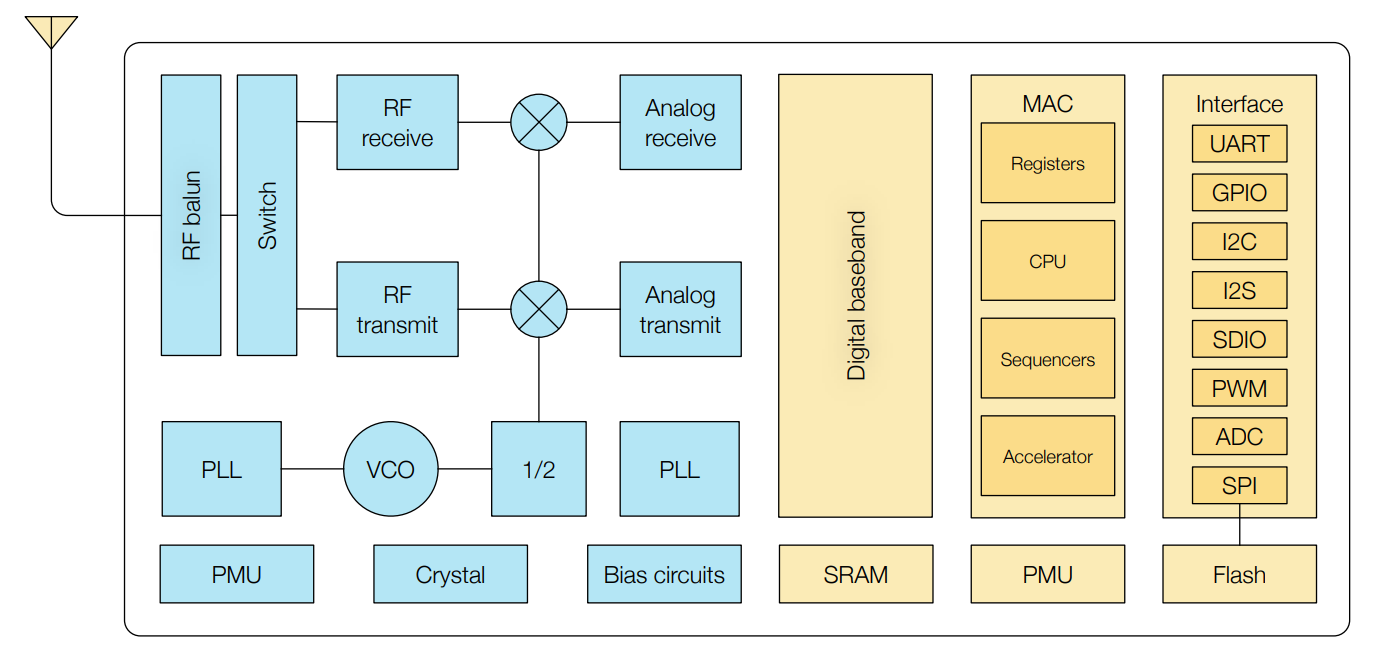
\includegraphics[width=150mm, keepaspectratio]{figures/esp8266funcdiag.png}
    \caption{Az ESP8266 funkcionális diagramja}
    \label{fig:TeXstudio}
\end{figure}

% különböző modul típusok
% elérhető lábszám
% alacsony ár
% iotban elterjedt, hasonló ellenfele
% Az előnyeihez sorolható, hogy alacsony fogyasztású és gyorsan tud váltani futó és alvó állapot között.

\section{ESPNOW}